\chapter{Funciones de dos variables}
En estudios anteriores, hemos revisado funciones de una variable $f: \mathbb{R} \rightarrow \mathbb{R}$,
en esta sección revisaremos funciones de dos variables es decir, $f: \mathbb{R}^{2} \rightarrow \mathbb{R}$,
las funciones dos variables permiten el estudio de la densidad de la tierra, la presión de un globo, ciertos modelos matemáticos están descritos por funciones de dos variables.\par
\section{Definición}
Recuperado de \cite{strang}.\par
Una función de dos variables $z=f(x, y)$ mapea cada par ordenado $(x, y)$ en un subconjunto $D$ del plano real $\mathbb{R}^{2}$ a un único número real $z$. El conjunto $D$ se llama dominio de la función. El rango de $f$ es el conjunto de todos los números reales $z$ que tiene al menos un par ordenado $(x, y) \in D$ tal que $f(x, y)=z$ como se muestra en la siguiente figura.\par
\begin{figure}[H]
    \centering
    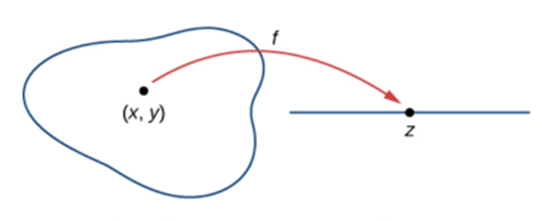
\includegraphics[width=9.5cm, height=5.5cm]{imagenes/NImagen1.png}
    \caption{El dominio de una función de dos variables consta de pares ordenados $(x, y)$.}
\end{figure}
\textbf{Nota:} Si una función $z=f(x, y)$ viene dada por una fórmula, asumimos que su dominio consta de todos los puntos $(x, y)$ para los cuales la fórmula tiene sentido, a menos que se especifique un dominio diferente.\par
\subsection{Gráfica de una función de dos variables}
La grafica de una función de dos variables es el conjunto de puntos $(\mathrm{x}, \mathrm{y}, \mathrm{z})$ tales que $z=f(x, y) y \quad x \in D$. Es decir,\par
$$
    \operatorname{Graf}(f)=\{(x, y, f(x, y)) \mid(x, y) \in D\}
$$
Tal que su representación seria.\par
\begin{figure}[H]
    \centering
    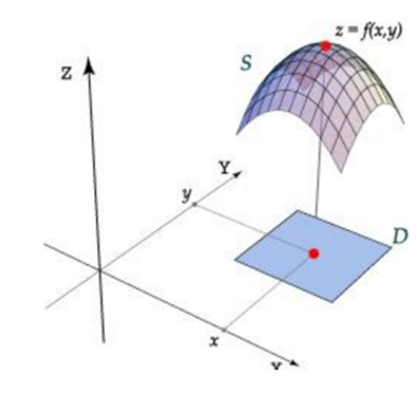
\includegraphics[width=9.5cm, height=7.5cm]{imagenes/Imagen4.png}
    \caption{Función de dos variables.}
\end{figure}
\newpage
\subsection{Ejemplo}

Representaciones geométricas de una tabla.\par
Recuperado de \cite{strang}, Suponga que la función $f$ está representada por la siguiente tabla:\par
\begin{table}[H]
    \centering
    \caption{Tabla de dos Entradas}
    \begin{tabular}{|c|c|c|c|c|}
        \hline                & $y=0$ & $y=1$ & $y=2$ & $y=3$ \\
        \cline { 2 - 5 }$x=0$ & 0     & 5     & 10    & 15    \\
        \cline { 2 - 5 }$x=1$ & 10    & 15    & 20    & 25    \\
        \hline$x=2$           & 20    & 25    & 30    & 35    \\
        \hline$x=3$           & 30    & 35    & 40    & 45    \\
        \hline
    \end{tabular}
    \bigskip
\end{table}

Geométricamente, podemos ver la información contenida en la tabla colocando primero un punto para cada $(x, y)$ en la tabla en el plano $x y$ de nuestro 3 -espacio\par

\begin{figure}[H]
    \centering
    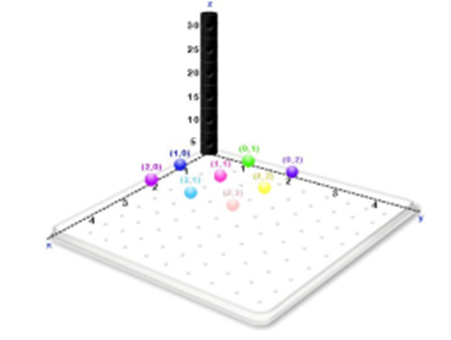
\includegraphics[width=7.5cm, height=7.5cm]{imagenes/NImagen2.png}
    \caption{Representación geométrica}
\end{figure}
\newpage
Entonces podemos elevar cada punto a su valor $z$ apropiado (altura) en 3 dimensiones.\par

\begin{figure}[H]
    \centering
    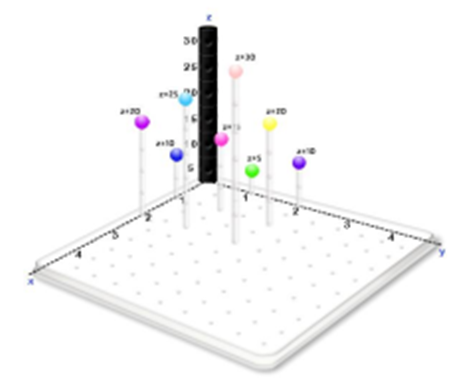
\includegraphics[width=7.5cm, height=7.5cm]{imagenes/Imagen3.png}
    \caption{Con su altura $z$}
\end{figure}

\subsection{Limites y Continuidad}
\section{Limite}
\textbf{Definición:} Sea $D$ un subconjunto de $\mathbb{R}^{n}$ y $f: D \rightarrow \mathbb{R}$, una función definida en $D$, y sea $a$ en un punto de acumulación de $D$. Decimos que el límite de una función $f$ cuando $x$ se acerca a $a$ es $L \in \mathbb{R}$, y lo escribiremos $\lim _{x \rightarrow a} f(x)=L$ si para cada $\epsilon>0$ hay un $\delta>0$ tal que $|f(x)-L|<\epsilon$ si $x \in D$ y $0<d(x, a)<\delta$.\par
Ademas se puede considerar las siguientes propiedades:\par
\begin{enumerate}
    \item Ley constante:\par
          $$
              \lim _{(x, y) \rightarrow(a, b)} c=c
          $$
    \item Leyes de identidad:\par
          $$
              \begin{aligned}
                   & \lim _{(x, y) \rightarrow(a, b)} x=a \\
                   & \lim _{(x, y) \rightarrow(a, b)} y=b
              \end{aligned}
          $$
    \item Ley de la suma:\par
          $$
              \lim _{(x, y) \rightarrow(a, b)}(f(x, y)+g(x, y))=L+M
          $$
    \item Ley de diferencia:\par
          $$
              \lim _{(x, y) \rightarrow(a, b)}(f(x, y)-g(x, y))=L-M
          $$
    \item Ley del múltiplo constante:\par
          $$
              \lim _{(x, y) \rightarrow(a, b)}(c f(x, y))=c L
          $$
    \item Ley del producto:\par
          $$
              \lim _{(x, y) \rightarrow(a, b)}(f(x, y) g(x, y))=L METRO
          $$
    \item Ley del cociente:\par
          $$
              \lim _{(x, y) \rightarrow(a, b)} \frac{f(x, y)}{g(x, y)}=\frac{L}{M} \text { para } M \neq 0
          $$
    \item Ley de potencia:\par
          $$
              \lim _{(x, y) \rightarrow(a, b)}(f(x, y))^{n}=L^{n}
          $$
          para cualquier entero positivo $n$.\par
    \item Ley de la raíz:
          $$
              \lim _{(x, y) \rightarrow(a, b)} \sqrt[n]{f(x, y)}=\sqrt[n]{L}
          $$
          para todo $L$ si $n$ es impar y positivo, y para $L \geq 0$ si $n$ es par y positivo.\par
\end{enumerate}
\section{Continuidad:}
\textbf{Definición:} Una función $f(x, y)$ es continua en un punto $(a, b)$ de su dominio si se cumplen las siguientes condiciones:
1. $f(a, b)$ existe.\par
2. $\lim _{(x, y) \rightarrow(a, b)} f(x, y)$ existe.\par
3. $\lim _{(x, y) \rightarrow(a, b)} f(x, y)=f(a, b)$.\par
\par
Intuitivamente podemos decir que una función continua de dos variables no tiene saltos.Consideremos el siguiente ejemplo para analizar la continuidad.\par
\textbf{Ejemplo:}\par
Consideramos la función:
$$
    f(x, y)= \begin{cases}\frac{x y^{2}}{x^{2}+y^{4}} & \text { si } x \neq 0 \\ 0 & \text { si } x=0\end{cases}
$$
Queremos comprobar que $f$ no es continua en el punto $(0,0)$. Para conseguirlo veremos que si nos acercamos a $(0,0)$ siguiendo trayectorias diferentes, obtenemos resultados también diferentes. Empezamos por las trayectorias más sencillas: las rectas. Una recta que pase por $(0,0)$ tiene la ecuación:
$$
    a x+b y=0,
$$
donde $a$ y $b$ son números fijos. A continuación estudiaremos dos casos diferentes:
a) Si $b=0$, entonces la recta es $x=0$, es decir, estamos observando la función a lo largo del eje $Y$. En este caso, tenemos que $f(0, y)=0$ para todo $y$, que es una función continua (al ser constante).
b) Si $b \neq 0$, tenemos que $y=-\frac{a}{b} x$. Definimos $c=-\frac{a}{b}$ tal que $y=c x$. El valor que toma la función en este punto es:
$$
    f(x, c x)= \begin{cases}\frac{c^{2} x^{3}}{x^{2}+c^{4} x^{4}} & \text { si } x \neq 0 \\ 0 & \text { si } x=0\end{cases}
$$
$$
    f(x, c x)= \begin{cases}\frac{c^{2} x^{3}}{x^{2}+c^{4} x^{4}} & \text { si } x \neq 0 \\ 0 & \text { si } x=0\end{cases}
$$
Esta función de una variable es continua para todo $c$ fijado, puesto que:
$$
    \lim _{x \rightarrow 0} f(x, c x)=c^{2} \lim _{x \rightarrow 0} \frac{x}{1+c^{4} x^{2}}=0 .
$$
Hemos visto que si nos acercamos a $(0,0)$ siguiendo trayectorias rectas, $f(x, y)$ es continua.
Por otro lado, para comprobar que $f$ no es continua en $(0,0)$, consideramos la trayectoria (parabólica) establecida por $x=y^{2}$. En este caso, la función de una variable que resulta es:
$$
    f\left(y^{2}, y\right)= \begin{cases}\frac{y^{4}}{y^{4}+y^{4}} & \text { si } y \neq 0 \\ 0 & \text { si } y=0\end{cases}
$$
es decir:
$$
    f\left(y^{2}, y\right)= \begin{cases}\frac{1}{2} & \text { si } y \neq 0 \\ 0 & \text { si } y=0\end{cases}
$$
que corresponde claramente a una función discontinua cuando $y=0$, lo cual implica, en particular, que la función $f(x, y)$ no puede ser continua en el punto $(0,0)$.